\documentclass[tikz,border=5pt]{standalone}
\usetikzlibrary{calc,patterns,angles,quotes}
\begin{document}
	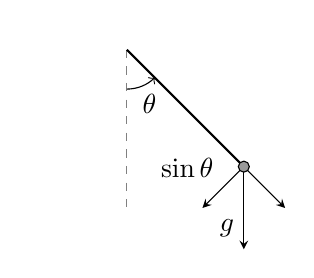
\begin{tikzpicture}[scale=0.7]
		% Increase the angle to make the image more square
		\pgfmathsetmacro{\Gvec}{1.5}
		\pgfmathsetmacro{\myAngle}{45}
		% calculate lengths of vector components
		\pgfmathsetmacro{\Gcos}{\Gvec*cos(\myAngle)}
		\pgfmathsetmacro{\Gsin}{\Gvec*sin(\myAngle)}
		
		\coordinate (centro) at (0,0);
		\draw[dashed,gray,-] (centro) -- ++ (0,-3) node (mary) [black,below]{$ $};
		\draw[thick] (centro) -- ++(270+\myAngle:3) coordinate (bob);
		\pic [draw, ->, "$\theta$", angle eccentricity=1.5] {angle = mary--centro--bob};
		\draw [-stealth] (bob) -- ($(bob)!-\Gcos cm!(centro)$)
		coordinate (gcos);
		\draw [-stealth] (bob) -- ($(bob)!\Gsin cm!90:(centro)$)
		coordinate (gsin)
		node[midway,above left] {$\sin\theta$};
		\draw [-stealth] (bob) -- ++(0,-\Gvec)
		coordinate (g)
		node[near end,left] {$g$};
		% Removed the entire pic command for the second angle
		\filldraw [fill=black!40,draw=black] (bob) circle[radius=0.1];
		
		% Tighter bounding box to eliminate whitespace
		\useasboundingbox (-1.8,-3.2) rectangle (1.8,0.4);
	\end{tikzpicture}
\end{document}